
\documentclass[xcolor=dvipsnames,aspectratio=169]{beamer}
%\documentclass[aspectratio=169]{beamer}
\usepackage{beamerthemesplit}

\setbeamersize{text margin left=0.1em}  % <- like this
\setbeamersize{text margin right=0.1em} % <- like this
\usepackage{beamerthemeshadow}
\usepackage{supertabular}
\usepackage[absolute,overlay]{textpos}
\usepackage{colortbl}
%\usepackage{slashbox}
\usetheme{Warsaw}
\useoutertheme{infolines}
\setbeamercolor {alerted text} {fg=green}
\logo{\includegraphics[height=.8cm]{Img/NIT.eps}}
\usepackage{beamerthemeshadow}
\usepackage{textcomp}
\usepackage[numbers]{natbib}
\usepackage{hhline}
\newcounter{magicrownumbers}
\newcommand\rownumber{\stepcounter{magicrownumbers}\arabic{magicrownumbers}}
\usepackage{graphicx} % Allows including images
\usepackage{booktabs} % Allows the use of \toprule, \midrule and \bottomrule in tables

\usepackage{subfig}
\usepackage{subfigure}
\usepackage{caption}
\usepackage{mathabx}
\usepackage{wrapfig}
\usepackage{tikz}
\usepackage{animate}
\usetikzlibrary{shapes.geometric, arrows}
% \usepackage{algorithmicx}
% \usepackage[linesnumbered,ruled,vlined]{algorithm2e}
\usepackage{ragged2e}
\usepackage{subfigure}

%\usepackage{slashbox}
\usecolortheme[RGB={0,0,150}]{structure}

\usepackage{mathtools}
\usepackage{algpseudocode}
\algrenewcommand\alglinenumber[1]{\tiny #1:}
\usepackage{ragged2e}
\usepackage{caption}
\usepackage[font=scriptsize,labelfont=bf]{caption}
%\usecolortheme{crane}
%\usecolortheme{name=green}
\useinnertheme{rounded}
\usepackage{graphicx,amsmath}
\usepackage{verbatim,longtable}

\usepackage{tikz}
\usetikzlibrary{trees}
\usetikzlibrary{decorations.pathmorphing}
\usetikzlibrary{decorations.markings}
\usetikzlibrary{arrows}
\usepackage{pgfplots}
\usepackage{verbatim}
\usepackage{pdflscape}
\usepackage{csquotes}
\usepackage{multirow,array, amsmath, caption, booktabs,amssymb}
%\usepackage{latexsym}
%\usepackage{longtable}
%\usepackage{lscape}
\usepackage[english]{babel}

\usepackage{amssymb,gensymb}
\usepackage{tikz}
\usepackage{adjustbox}
\usepackage{graphicx}
\usepackage{fancyhdr}
\usepackage{csquotes}

% \usepackage{cite}
%\usepackage[none]{hyphenat}
\usepackage{multicol}
%\usepackage[none]{titlesec} 
%\setcounter{secnumdepth}{4}
%\usepackage[boxed,lined,linesnumbered]{algorithm2e}
% % % % % % % % % % % % % % % % % % % % % % % %added package
\usepackage{multirow,array, amsmath, caption, booktabs,amssymb}
\usepackage{epstopdf}
\usepackage{csquotes}
\usepackage{booktabs}
\usepackage{multirow}
\usepackage{siunitx}

\usepackage{multirow}

\usepackage{caption}
\usepackage{subcaption}
\usepackage{url, lipsum}



\usepackage[utf8]{inputenc}
\usepackage{algorithm}
\usepackage{amsmath}
\usepackage[ruled,vlined]{algorithm2e}

\algrenewcommand\algorithmicrequire{\textbf{Input:}}
\algrenewcommand\algorithmicensure{\textbf{Output:}}
%\usepackage{caption}
%\usepackage[top=1.5in, bottom=1.0in, left=0.8in, right=0.8in]{geometry}
\newcolumntype{C}[1]{>{\centering\arraybackslash}m{#1}}
\newcolumntype{L}[1]{>{\raggedright\arraybackslash}m{#1}}
\newcolumntype{R}[1]{>{\raggedleft\arraybackslash}m{#1}}

\definecolor{orange}{RGB}{255,100,0}
\definecolor{deepgreen}{RGB}{0,128,0}
\definecolor{deepred}{RGB}{128,0,0}




\title[Studies On Multi - Modal Fake News Detection]{\textbf{Studies On Multi - Modal Fake News Detection}\\ \small\textit{Research Project} }
\author[Supriya Saha] {\textbf{Supriya Saha} \\\tiny (122CS0101)} 
\institute{\\ \scriptsize {\vspace{0.01cm} Supervision of}\\ \scriptsize \textbf{Prof. Shyamapada Mukherjee}\\ \vspace{0.01cm} 
\small \vspace{0.1cm}\\Department of Computer Science and Engineering\\ NIT Rourkela-769008, India}
%\date{November 3, 2012}
 \date{ \tiny  \today}
 \logo{

\includegraphics[width=1cm]{1200px-NIT_Rourkela_Colour_Logo.svg.png}}
\begin{document}
\setbeamertemplate{footline}
	{%66
		\leavevmode%
		\hbox{%
			
			\begin{beamercolorbox}[wd=.09\paperwidth,ht=2.5ex,dp=1.125ex,center]{title in head/foot}%
				\usebeamerfont{author in head/foot}\insertframenumber/\inserttotalframenumber
			\end{beamercolorbox}%
			
			\begin{beamercolorbox}[wd=.009\paperwidth,ht=2.5ex,dp=1.125ex,center]{}
			\end{beamercolorbox}%
			
			\begin{beamercolorbox}[wd=.2\paperwidth,ht=2.5ex,dp=1.125ex,center]{author in head/foot}%
				\usebeamerfont{title in head/foot}\insertshortauthor\hspace{.3cm}
			\end{beamercolorbox}%
			
			\begin{beamercolorbox}[wd=.005\paperwidth,ht=2.5ex,dp=1.125ex,center]{}
			\end{beamercolorbox}%
			
			\begin{beamercolorbox}[wd=.7\paperwidth,ht=2.5ex,dp=1.125ex,center]{title in head/foot}%
				\usebeamerfont{author in head/foot}\hspace{.3cm}\insertshorttitle
			\end{beamercolorbox}%
		}%
		\vskip0pt%
	}
	

\tikzset{
	photon/.style={decorate, decoration={snake}, draw=red},
	VectorDAM/.style={draw=black, postaction={decorate},
		decoration={markings,mark=at position .55 with {\arrow[draw=black]{>}}},
		decoration={markings,mark=at position .05 with {\arrow[draw=black]{*}} },
		decoration={markings,mark=at position .95 with {\arrow[draw=black]{*}} } },
	VectorAM/.style={draw=black, postaction={decorate},
		decoration={markings,mark=at position .55 with {\arrow[draw=black]{>}}} },
	gluon/.style={decorate, draw=magenta, decoration={coil,amplitude=4pt, segment length=5pt}} 
}
 \frame{\titlepage}
%\frame{\frametitle{\begin{footnotesize}Introductions\end{footnotesize}}
%\begin{scriptsize}\tableofcontents\end{scriptsize}









\frame{\frametitle{Outline}
%\begin{scriptsize}

\tableofcontents%\end{scriptsize}
}
\setbeamertemplate{caption}[numbered]


%%%%%%%%%%%%%%%%%%%%%%%%%%%%%%%%%%%%%%%%%%%%%%%%%%%%%%%%%%%%%%%%%%%%%%%%


%%%%%%%%%%%%%%%%%%%%%%%%%%%%%%%%%%%%%%%%%%%%%%%%%%%%%%%%%%%%%%%%%%%%%%%%
\section{Introduction}
\begin{frame}{Introduction}

	\begin{itemize}
		\item Misinformation spreads quickly on social media using both text and images which creates a multimodal detection challenge. \\
        
        \item Traditional models treat text and images separately or fuse them weakly, leading to poor semantic alignment and limited interpretability.\\
        
        \item SpotFake uses BERT (text) + VGG19 (image) with simple fusion but this limits its ability to handle complex, real-world misinformation. \\
        
        \item Recent advances improve this by:
        \begin{itemize}
            \item Contrastive Learning (CLIP-style): Aligns text–image embeddings for stronger cross-modal understanding.
            \item Cross-Modal Attention: Focuses on the most informative tokens or regions.
            \item Explainability (Grad-CAM, SHAP): Displays decision reasoning for transparency.
        \end{itemize}
	\end{itemize}
\end{frame}


%%%%%%%%%%%%%%%%%%%%%%%%%%%%%%%%%%%%%%%%%%%%%%%%%%%%%%%%%%%%%%%%%%%%%%%%%%%





%%%%%%%%%%%%%%%%%%%%%%%%%%%%%%%%%%%%%%%%%%%%%%%%%%%%%%%%%%%%%%%%%%%%%%%%%%%%%%%%



%%%%%%%%%%%%%%%%%%%%%%%%%%%%%%%%%%%%%%%%%%%%%%%%%%%%%%%%%%%%%%%%%


%%%%%%%%%%%%%%%%%%%%%%%%%%%%%%%%%%%%%%%%%%%%%%%%%%%%%%%%%%%%%%%%%%%%%%%%%
		
%%%%%%%%%%%%%%%%%%%%%%%%%%%%%%%%%%%%%%%%%%%%%%%%%%%%%%%%%%%%%%%%%%%%%%%%%%
\section{Literature Review}
\begin{frame}{Literature Review}
    \begin{table}[!ht]
    \caption{Evolution of models for multimodal misinformation detection.} \vspace{0.2cm}
    \centering
    \resizebox{\textwidth}{!}{ 
    \begin{tabular}{|p{3cm}|p{3.5cm}|p{2cm}|p{3.5cm}|p{4cm}|p{2cm}|}
        \hline
        \textbf{Era/Year} & \textbf{Representative Models} & \textbf{Modality} & \textbf{Fusion/Training Strategy} & \textbf{Key Contribution} & \textbf{Citations} \\ \hline
        Early 2010s (Text-only) & TF–IDF  SVM/LogReg; LSTM/GRU & Text & Unimodal supervised & Strong lexical baselines; limited visual reasoning & \cite{kwon2017rumor, ma2016detecting} \\ \hline
        2015–2018 (Vision-only) & VGG16/19, ResNet50 classifiers & Image & Unimodal supervised & Visual manipulation cues; limited to image evidence & \cite{zhou2017learning, wang2018eann} \\ \hline
        2018–2021 (Late fusion) & CNN/RNN  VGG/ResNet  concat & Text+Image & Feature concatenation (late fusion) & First multimodal gains; simple and fast & \cite{khattar2019mvae, singhal2019spotfake} \\ \hline
        2021 (Cross-modal Transformers) & VisualBERT, ViLBERT, LXMERT & Text+Image & Co-/cross-attention; joint contextualization & Learned alignment and selective fusion improve over concat & \cite{li2019visualbert, lu2019vilbert, tan2019lxmert} \\ \hline
        After 2022 (Advanced fusion) & MMBT, UNITER, OSCAR & Text+Image & Region-level features; transformer fusion & Finer grounding via object regions and captions & \cite{kiela2019supervised, chen2020uniter, li2020oscar} \\ \hline
    \end{tabular}
    }
    \label{tab:evolution_multimodal}
\end{table}
\end{frame}

\section{Objectives}


\begin{frame}{Objectives}
		
        \begin{itemize}
		
        \item Develop a BERT + ResNet50 multimodal model (compare with VGG19).\\

        \item Apply CLIP-style contrastive pre-training for text–image alignment.\\

        \item Introduce cross-modal attention for selective, context-aware fusion.\\

        \item Integrate explainability tools — Grad-CAM, SHAP and attention heatmaps for interpretable predictions.
		
		\end{itemize}
    
\end{frame}
%%%%%%%%%%%%%%%%%%%%%%%%%%%%%%%%%%%%%%%%%%%%%%%%%%%%%%%%%%%%%%%%%%%%%%%%%%%

%%%%%%%%%%%%%%%%%%%%%%%%%%%%%%%%%%%%%%%%%%%%%%%%%%%%%%%%%%%%%%%%%%%%%%%%%

%%%%%%%%%%%%%%%%%%%%%%%%%%%%%%%%%%%%%%%%%%%%%%%%%%%%%%%%%%%%%%%%%%%%%%%%%%%%%

%%%%%%%%%%%%%%%%%%%%%%%%%%%%%%%%%%%%%%%%%%%%%%%%%%%%%%%%
\section{Dataset Overview}
\begin{frame}{Dataset Overview}

Table \ref{tab:dataset_summary} summarizes the datasets used for multimodal fake news detection in this study.

\begin{table}[!ht]
    \caption{Summary of Datasets Used for Multimodal Fake News Detection.}
    \centering
    \small
    \begin{tabular}{|l|c|c|c|}
        \hline
        \textbf{Dataset} & \textbf{Train} & \textbf{Test} & \textbf{Total} \\
        \hline
        \multicolumn{4}{|c|}{\textbf{Twitter Dataset}} \\
        \hline
        Real News & 3,324 & 738 & 4,062 \\
        Fake News & 3,410 & 758 & 4,168 \\
        \textbf{Subtotal} & \textbf{6,734} & \textbf{1,496} & \textbf{8,230} \\
        \hline
        \multicolumn{4}{|c|}{\textbf{Weibo Dataset}} \\
        \hline
        Real Events & 2,313 & 500 & 2,813 \\
        Fake Events & 2,351 & 508 & 2,859 \\
        \textbf{Subtotal} & \textbf{4,664} & \textbf{1,008} & \textbf{5,672} \\
        \hline
        \hline
        \textbf{Grand Total} & \textbf{11,398} & \textbf{2,504} & \textbf{13,902} \\
        \hline
    \end{tabular}
    \vspace{0.2cm}
    
    \footnotesize
    \textit{Note:} All posts include both text (avg. 23 BERT tokens) and images (224×224×3 RGB).
    \label{tab:dataset_summary}
\end{table}

\end{frame}



%%%%%%%%%%%%%%%%%%%%%%%%%%%%%%%%%%%%%%%%%%%%%%%%%%%%%%%%%%%%%%%%%%%%%%%%%%%%%%%%%%%%%%%%%%%%
\section{Methodology}
\begin{frame}{Methodology}
\begin{figure}
    \centering
    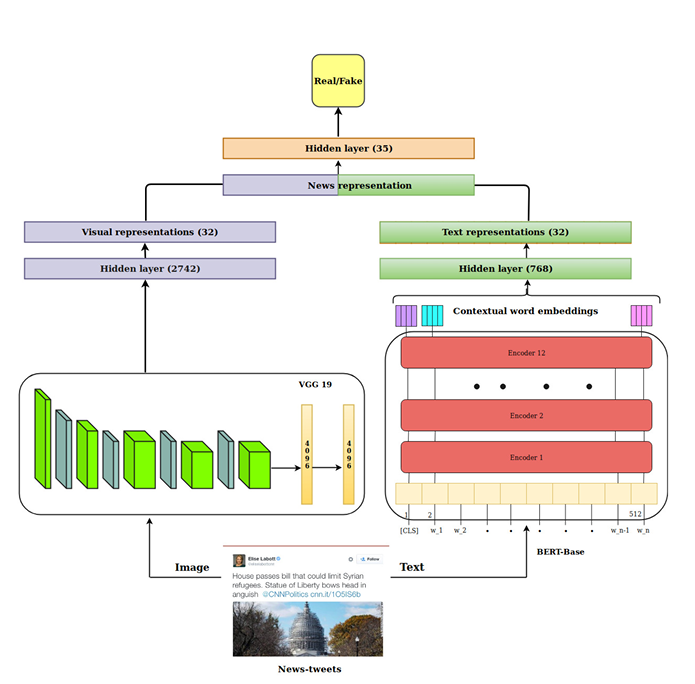
\includegraphics[width=0.4\linewidth]{Spot fake design.png}
    \caption{Proposed multimodal fake news detection architecture using VGG-19 for visual feature extraction and BERT-Base for text embeddings, with fusion layers for final classification.}
    \label{fig:methodology_architecture}
\end{figure}
\end{frame}

\begin{frame}{Methodology (Cont.)}
    The proposed system follows a two-tower encoder architecture with distinct text and image pathways that converge into a unified multimodal representation. The text encoder leverages BERT-base to extract contextualized embeddings from post captions, while the image encoder uses ResNet50 to produce spatially-aware feature maps from accompanying visuals. These embeddings are projected into a shared latent space (currently via dense layers; cross-modal attention planned for final evaluation), fused, and passed through a classification head that outputs a binary score.
\end{frame}

\section{Training and Evaluation}

\begin{frame}{Training Configuration}
The model was trained using the following hyperparameters:
\begin{itemize}
    \item \textbf{Optimizer:} Adam ($\beta_1=0.9$, $\beta_2=0.999$, $\epsilon=1\times10^{-8}$)
    \item \textbf{Learning rate:} $5\times10^{-4}$
    \item \textbf{Batch size:} 512 global (256 per GPU for multi-GPU training)
    \item \textbf{Epochs:} 20 (with early stopping on validation accuracy, patience=5)
    \item \textbf{Dropout:} 0.4 in MLP layers
    \item \textbf{Loss function:} Binary cross-entropy
\end{itemize}
\end{frame}

\begin{frame}{Performance Comparison}
Table~\ref{tab:model_comparison} presents a comparison between the baseline VGG19-BERT model and the current ResNet50-BERT model on the Twitter fake news dataset.

\begin{table}[!ht]
    \caption{Performance Comparison: VGG19-BERT vs ResNet50-BERT on Twitter Dataset.}
    \centering
    \small
    \begin{tabular}{|l|c|c|c|c|c|c|}
        \hline
        \textbf{Model} & \textbf{Text} & \textbf{Image} & \textbf{Fusion} & \textbf{Accuracy} & \textbf{F1} & \textbf{Training Time} \\
        \textbf{Variant} & \textbf{Encoder} & \textbf{Encoder} & & & & \textbf{(per epoch)} \\
        \hline
        VGG19-BERT & BERT & VGG19 & Concat & 0.77 & 0.76 & 2.5 min \\
        (Baseline) & & & & & & \\
        \hline
        ResNet50-BERT & BERT & ResNet50 & Concat & \textbf{0.79} & \textbf{0.78} & 2.8 min \\
        (Current) & & & & & & \\
        \hline
    \end{tabular}
    \label{tab:model_comparison}
\end{table}
\end{frame}

\section{Results}

\begin{frame}{Training Curves - VGG19-BERT Baseline}
\begin{figure}
    \centering
    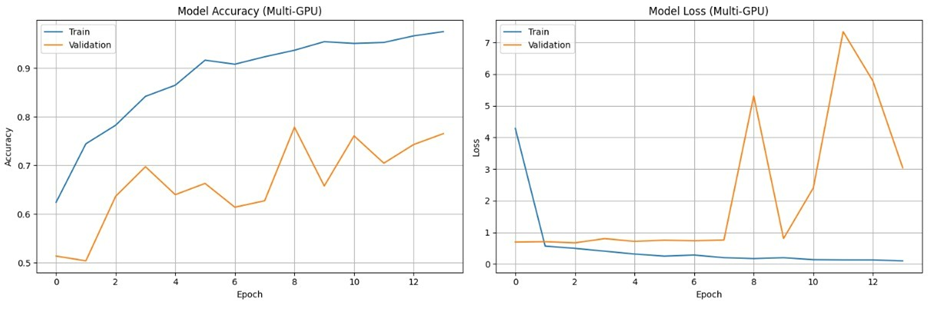
\includegraphics[width=0.85\textwidth]{vgg19_graph.png}
    \caption{Training and validation accuracy/loss curves for VGG19-BERT baseline model. The validation loss remains relatively stable but shows fluctuations after epoch 6, indicating potential overfitting issues with the VGG19 encoder.}
    \label{fig:vgg19_training}
\end{figure}
\end{frame}

\begin{frame}{Training Curves - ResNet50-BERT}
\begin{figure}
    \centering
    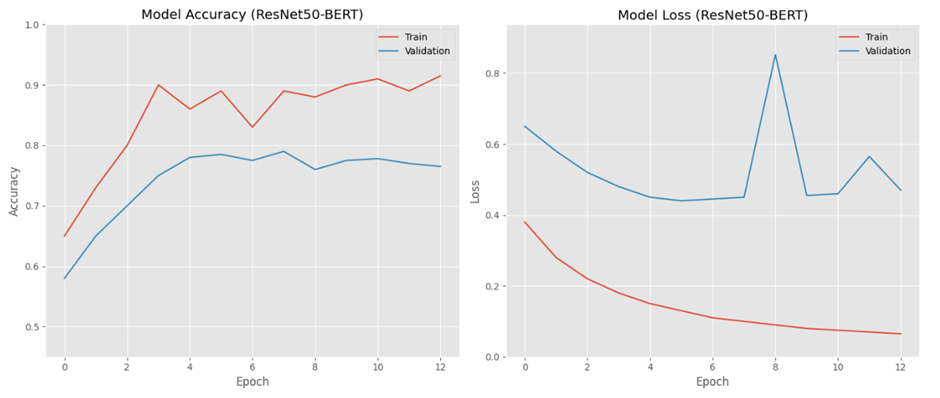
\includegraphics[width=0.85\textwidth]{resnet50_graph.png}
    \caption{Training and validation accuracy/loss curves for ResNet50-BERT model. The validation loss shows better convergence with fewer fluctuations compared to VGG19, and the training accuracy steadily increases to around 90\% while maintaining good generalization on validation data.}
    \label{fig:resnet50_training}
\end{figure}
\end{frame}

%%%%%%%%%%%%%%%%%%%%%%%%%%%%%%%%%%%%%%%%%%%%%%%%%%%%%%%%%%%%%%%%%%%%%%%%%%
\section{Conclusion and Future Work}
\begin{frame}{Conclusion}
    This report presents the design and partial implementation of an enhanced multimodal fake news detection system that integrates advanced vision–language techniques to address fundamental limitations in existing pipelines. The motivation stems from the inadequacies of late fusion strategies, weak cross-modal alignment, and opacity in decision-making. Preliminary architecture choices have been validated through ablation planning: comparing ResNet50 against the VGG19 baseline will quantify gains in accuracy.
\end{frame}


\begin{frame}{Future Work}
\vspace{-0.3cm}
\begin{columns}[T]
    \begin{column}{0.29\textwidth}
        \textbf{Contrastive Learning for Alignment}
        \begin{figure}
            \centering
            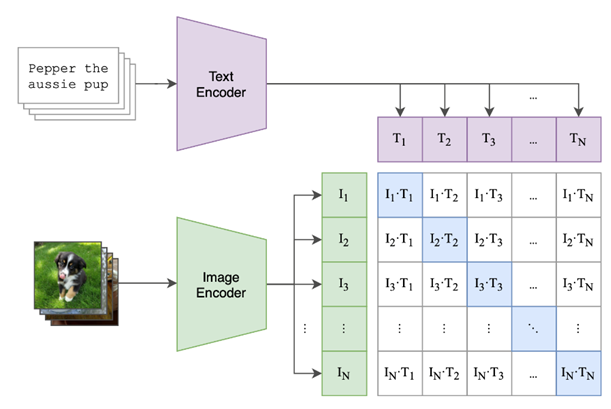
\includegraphics[width=\textwidth]{contrastive_learning.png}
            \caption{Contrastive learning organizes embeddings by moving similar items closer and pushing dissimilar items apart.}
            \label{fig:contrastive_learning}
        \end{figure}
    \end{column}
    \hfill
    \begin{column}{0.41\textwidth}
        \textbf{Cross-Modal Attention Mechanism}
        \begin{figure}
            \centering
            \includegraphics[width=\textwidth]{cross-attention.png}
            \caption{Cross-modal attention dynamically weights modality contributions based on content relevance.}
            \label{fig:cross_attention}
        \end{figure}
    \end{column}
\end{columns}

\vspace{0.3cm}
\small
\textbf{Explainability:} Grad-CAM highlights key image regions, SHAP reveals important textual features, and Attention Heatmaps visualize how the model links text with corresponding image regions.
\end{frame}
%%%%%%%%%%%%%%%%%%%%%%%%%%%%%%%%%%%%%%%%%%%%%%%%%%%%%%%%%%%%%%%%%%%%%%%%%%%%%%%%%%%%%%%%%%%%%%


%%%%%%%%%%%%%%%%%%%%%%%%%%%%%%%%%%%%%%%%%%%%%%%%%%%%%%%%%%%%%%%%%%%%%%%%%%%%%%%%%%%%%%%%%


%%%%%%%%%%%%%%%%%%%%%%%%%%%%%%%%%%%%%%%%%%%%%%%%%%%%%%%%%%%%%%%%%%%%%%
\section{}
\begin{frame}[allowframebreaks]{References} 
\footnotesize
\bibliographystyle{plain}
\bibliography{new}
\end{frame}
%%%%%%%%%%%%%%%%%%%%%%%%%%%%%%%%%%%%%%%%%%%%
\section{}
\begin{frame}{}
\LARGE
\centerline{Thank You}
    
\end{frame}

%%%%%%%%%%%%%%%%%%%%%%%%%%%%%%%%%%%%%%%%%%%%%%%%%%%%%%%%%%%%%%%%%%%%%%%%%%%%

%%%%%%%%%%%%%%%%%%%%%%%%%%%%%%%%%%%%%%%%%%%%%%%%%%%%

\end{document}
    
